\documentclass[11pt]{article}

%% MinionPro fonts 
%\usepackage[lf]{MinionPro}
%\usepackage{MnSymbol}
\usepackage{microtype}

%% Margins
\usepackage{geometry}
\geometry{verbose,letterpaper,tmargin=1in,bmargin=1in,lmargin=1in,rmargin=1in}

%% Other packages
\usepackage{amsmath}
\usepackage{amsthm}
\usepackage{amsfonts}
\usepackage[shortlabels]{enumitem}
\usepackage{titlesec}
\usepackage{soul}
\usepackage{tikz}
\usepackage{mathtools}
\usepackage{pgfplots}
\usepackage{tikz-3dplot}
\usepackage{algorithmic}
\usepackage[export]{adjustbox}
\usepackage{tcolorbox}
\usepackage{mathrsfs}
\usepackage{multicol}
\usepackage{framed}
%\usepackage{optprog}


%% Paragraph style settings
\setlength{\parskip}{\medskipamount}
\setlength{\parindent}{0pt}

%% Change itemize bullets
\renewcommand{\labelitemi}{$\bullet$}
\renewcommand{\labelitemii}{$\circ$}
\renewcommand{\labelitemiii}{$\diamond$}
\renewcommand{\labelitemiv}{$\cdot$}

%% Colors
\definecolor{rred}{RGB}{204,0,0}
\definecolor{ggreen}{RGB}{0,145,0}
\definecolor{yyellow}{RGB}{255,185,0}
\definecolor{bblue}{rgb}{0.2,0.2,0.7}
\definecolor{ggray}{RGB}{190,190,190}
\definecolor{ppurple}{RGB}{160,32,240}
\definecolor{oorange}{RGB}{255,165,0}

%% Shrink section fonts
\titleformat*{\section}{\normalsize\bf}
\titleformat*{\subsection}{\normalsize\bf}
\titleformat*{\subsubsection}{\normalsize\it}

% %% Compress the spacing around section titles
\titlespacing*{\section}{0pt}{1.5ex}{0.75ex}
\titlespacing*{\subsection}{0pt}{1ex}{0.5ex}
\titlespacing*{\subsubsection}{0pt}{1ex}{0.5ex}

%% amsthm settings
\theoremstyle{definition}
\newtheorem{problem}{Problem}
\newtheorem{example}{Example}
\newtheorem*{theorem}{Theorem}
\newtheorem*{bigthm}{Big Theorem}
\newtheorem*{biggerthm}{Bigger Theorem}
\newtheorem*{bigcor1}{Big Corollary 1}
\newtheorem*{bigcor2}{Big Corollary 2}

%% tikz settings
\usetikzlibrary{calc}
\usetikzlibrary{patterns}
\usetikzlibrary{decorations}
\usepgfplotslibrary{polar}

%% algorithmic setup
\algsetup{linenodelimiter=}
\renewcommand{\algorithmiccomment}[1]{\quad// #1}
\renewcommand{\algorithmicrequire}{\emph{Input:}}
\renewcommand{\algorithmicensure}{\emph{Output:}}

%% Answer box macros
%% \answerbox{alignment}{width}{height}
\newcommand{\answerbox}[3]{%
  \fbox{%
    \begin{minipage}[#1]{#2}
      \hfill\vspace{#3}
    \end{minipage}
  }
}

%% \answerboxfull{alignment}{height}
\newcommand{\answerboxfull}[2]{%
  \answerbox{#1}{6.38in}{#2} 
}

%% \answerboxone{alignment}{height} -- for first-level bullet
\newcommand{\answerboxone}[2]{%
  \answerbox{#1}{6.0in}{#2} 
}

%% \answerboxtwo{alignment}{height} -- for second-level bullet
\newcommand{\answerboxtwo}[2]{%
  \answerbox{#1}{5.8in}{#2}
}

%% special boxes
\newcommand{\wordbox}{\answerbox{c}{1.2in}{.7cm}}
\newcommand{\catbox}{\answerbox{c}{.5in}{.7cm}}
\newcommand{\letterbox}{\answerbox{c}{.7cm}{.7cm}}

%% Miscellaneous macros
\newcommand{\tstack}[1]{\begin{multlined}[t] #1 \end{multlined}}
\newcommand{\cstack}[1]{\begin{multlined}[c] #1 \end{multlined}}
\newcommand{\ccite}[1]{\only<presentation>{{\scriptsize\color{gray} #1}}\only<article>{{\small [#1]}}}
\newcommand{\grad}{\nabla}
\newcommand{\ra}{\ensuremath{\rightarrow}~}
\newcommand{\maximize}{\text{maximize}}
\newcommand{\minimize}{\text{minimize}}
\newcommand{\subjectto}{\text{subject to}}
\newcommand{\trans}{\mathsf{T}}
\newcommand{\bb}{\mathbf{b}}
\newcommand{\bx}{\mathbf{x}}
\newcommand{\bc}{\mathbf{c}}
\newcommand{\bd}{\mathbf{d}}

%% LP format
%    \begin{align*}
%      \maximize \quad & \mathbf{c}^{\trans} \mathbf{x}\\
%      \subjectto \quad & A \mathbf{x} = \mathbf{b}\\
%                       & \mathbf{x} \ge \mathbf{0}
%    \end{align*}

%Space between rows:
%\def\arraystretch{2.2}
%
%Space between columns:
%\arraycolsep=1.4pt


%% Redefine maketitle
\makeatletter
\renewcommand{\maketitle}{
  \noindent SA405 -- AMP \hfill Rader \S 13.1  \\

  \begin{center}\Large{\textbf{\@title}}\end{center}
}
\makeatother

%% ----- Begin document ----- %%
\begin{document}
  
\title{Lesson 16.  IP Formulations, Part 2}

\maketitle

%%%
\section{Today}
\renewcommand\labelitemi{--}
\begin{itemize}
\item  Convex Hull Formulations (\emph{Ideal} Formulations)
\item  IP Bounds
\end{itemize}

\section{Convex Hull Formulations} 

\subsection{Convex sets review}
Recall from SA305:
\begin{tcolorbox}
A region in $n$-dimensions is \textbf{convex} if for \emph{any 2 points}, $\textbf{x}$ and $\textbf{w}$, in the region, the line connecting $\textbf{x}$ and $\textbf{w}$ is \emph{completely} contained inside the region.
\end{tcolorbox}

\begin{problem} Draw a 2-dimensional example for each.
 \begin{enumerate}[(a)]
\item A region that is convex.
\item A region is not convex.  Illustrate a pair of points $\textbf{x}$ and $\textbf{w}$ in the region that demonstrate that the region is not convex.
\end{enumerate}
\answerbox{c}{.5\textwidth}{2in} \answerbox{c}{.5\textwidth}{2in}
\end{problem}

This is an important property for the simplex algorithm:
\begin{tcolorbox}
The feasible region of an LP is a convex set. 
\end{tcolorbox}

\textbf{Question:}  Is the feasible region of any IP convex?

\answerboxfull{c}{.5in}



\subsection{Convex Hull Formulations}

\begin{tcolorbox}
The \textbf{convex hull} of a set of integer feasible solutions is the \textbf{smallest convex set} that contains all of the points. 
\end{tcolorbox}

For example, we saw two different formulations for the same problem in the last lesson.  The inner formulation (below), is the convex hull formulation of the integer feasible region to the IP problem described by both formulations.  

\begin{minipage}{0.4\textwidth}
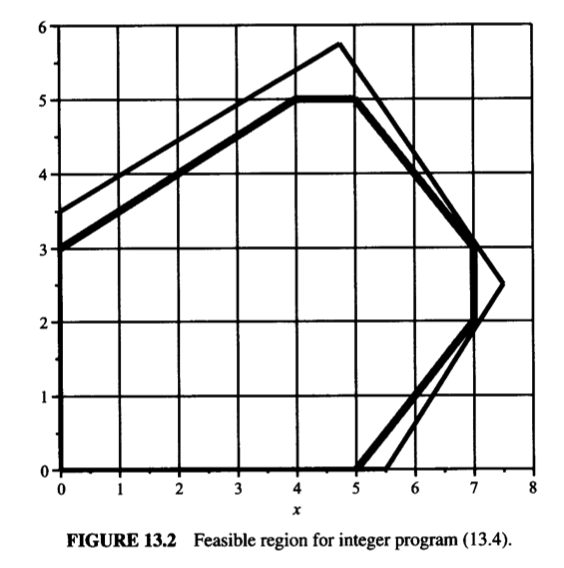
\includegraphics[width=0.7\textwidth]{formulation_ideal}
\end{minipage}
\begin{minipage}{0.6\textwidth}
\begin{itemize}
\item Note that \emph{all} linear formulations are necessarily convex.
\item It is the \emph{smallness} of the inner formulation that makes it the \emph{convex hull}. 
\item Notice that all corner points are integer points in the convex hull formulation.
\end{itemize}
\end{minipage}

\bigskip
\begin{problem}
Sketch the convex hull of the each of the following three collections of points.

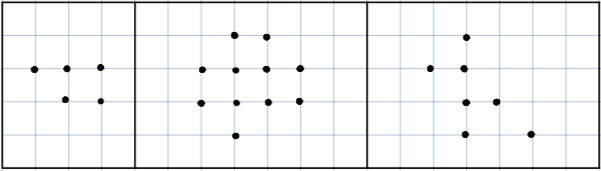
\includegraphics[width=.8\textwidth]{convex_hull_practice}
\end{problem}

\bigskip
%%%

\begin{problem} A formulation for a set of feasible integer solutions is pictured on the left.  The integer solutions are highlighted on the right.  Sketch the \textbf{convex hull formulation} of this set of solutions.

\vspace{0.5cm}
\begin{center}
\begin{minipage}{6.5in}
\centering
\raisebox{-0.5\height}{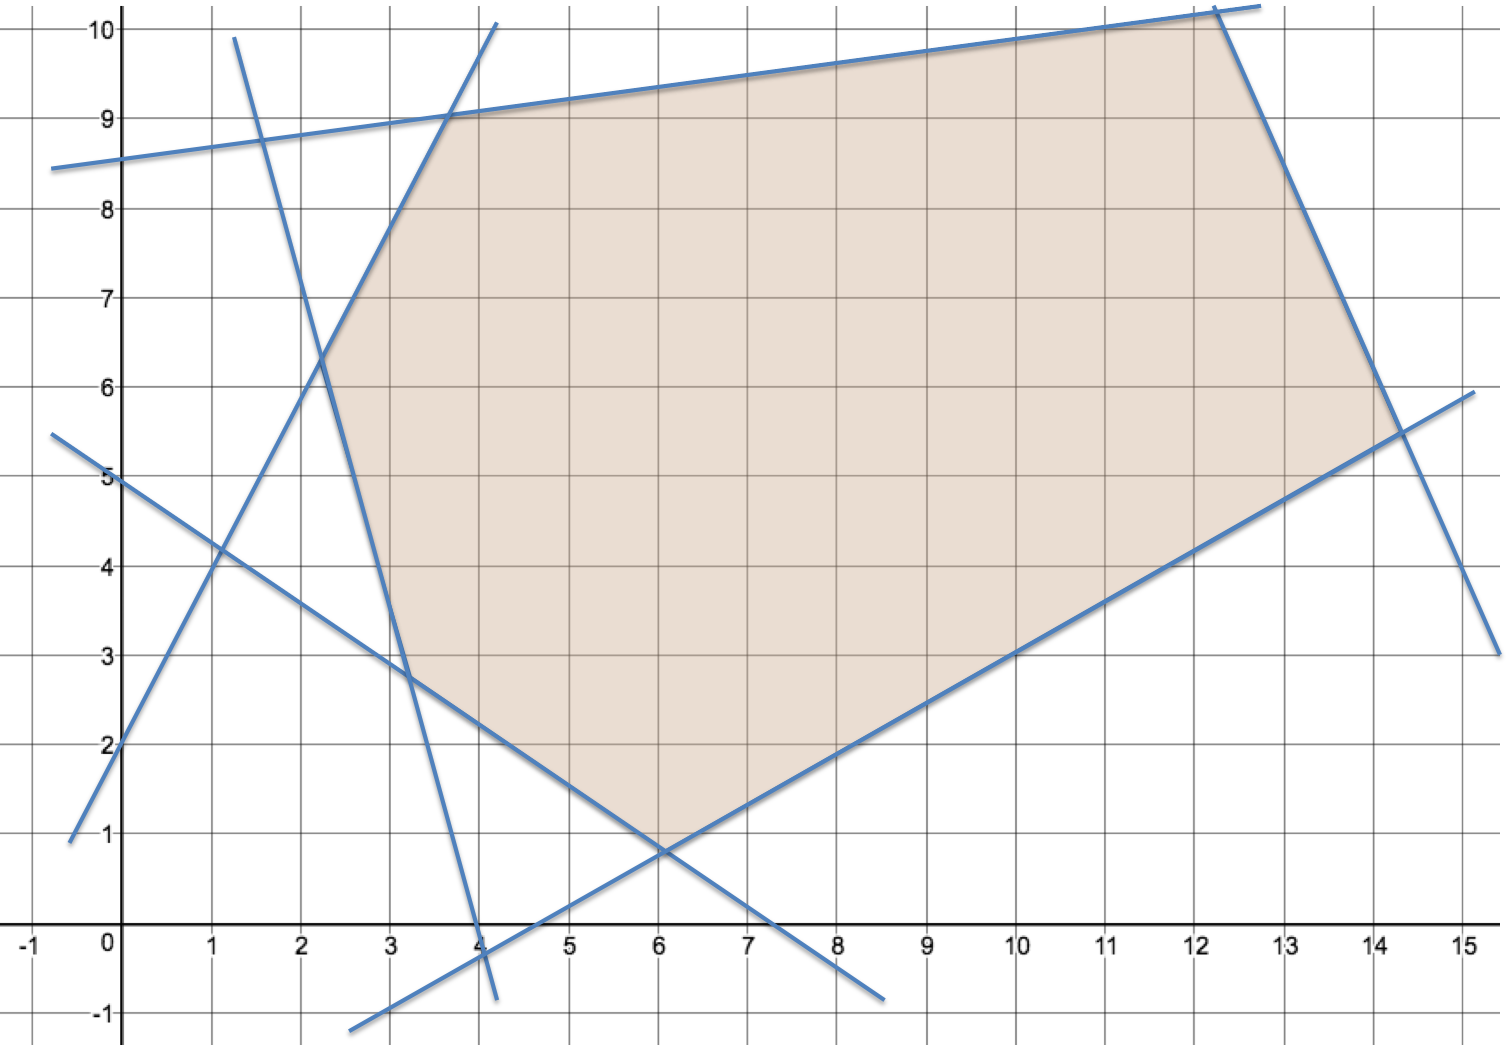
\includegraphics[width=0.35\textwidth]{convexhull_problem}}
\hspace*{0.2in}
\raisebox{-0.5\height}{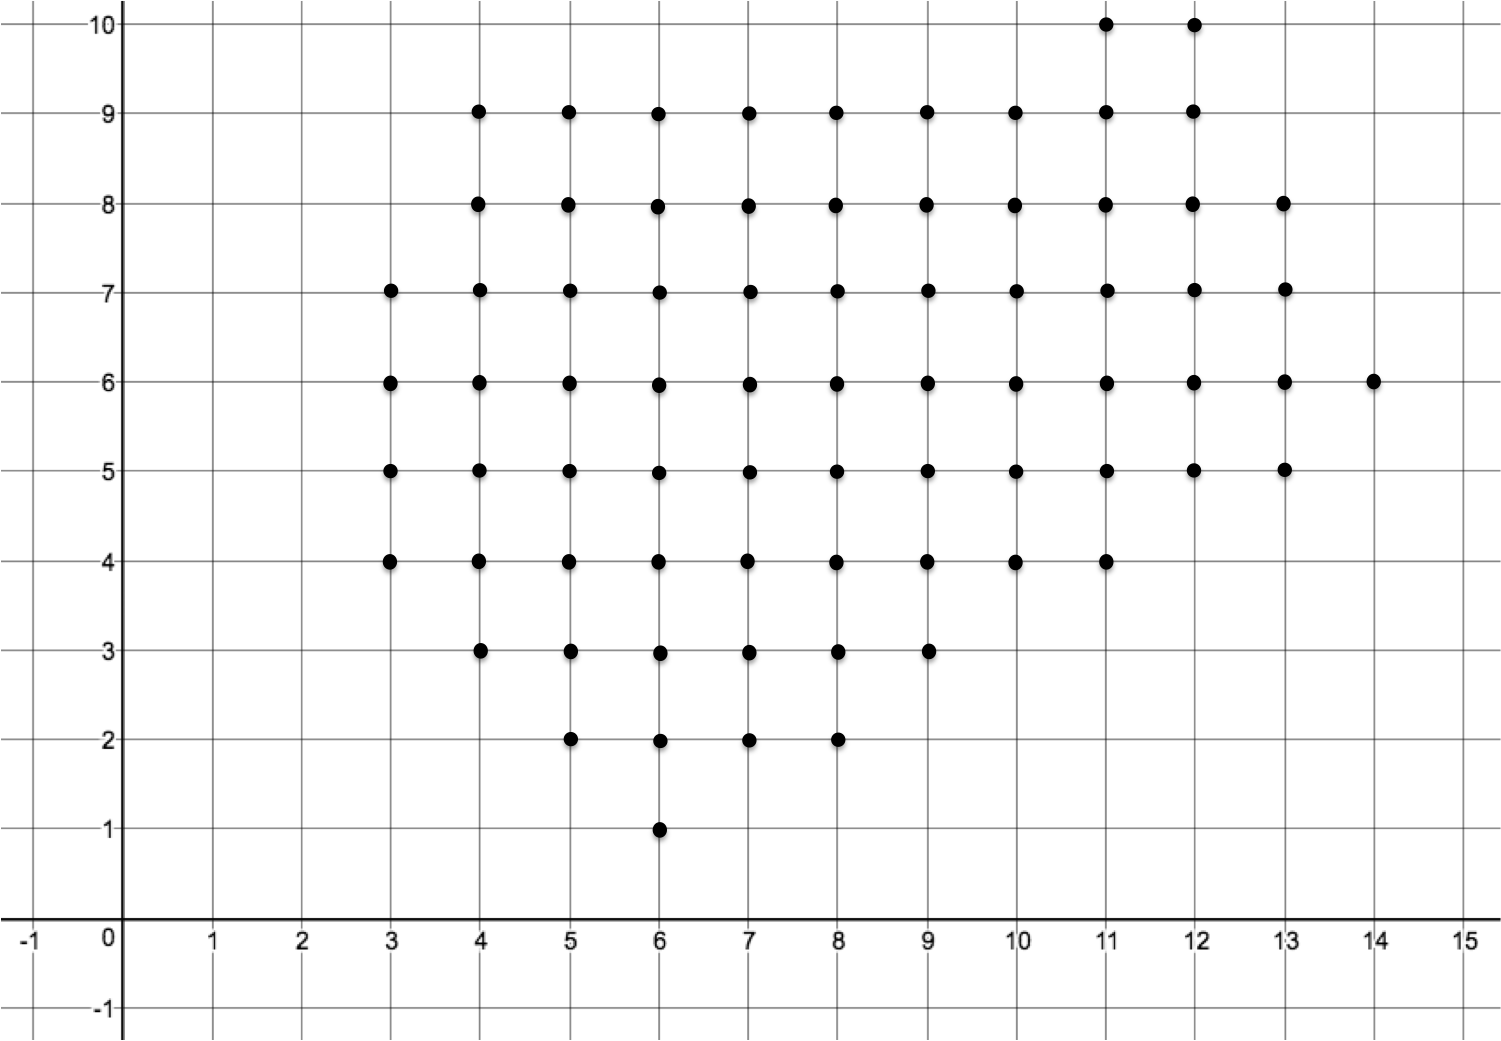
\includegraphics[width=0.6\textwidth]{convexhull_find}}
\end{minipage}
\end{center}
\end{problem}

\begin{tcolorbox}
The \textbf{convex hull formulation} of a finite set of integer feasible solutions is considered to be the \textbf{``ideal''} formulation.
\end{tcolorbox}

Why?

\answerboxfull{c}{2cm}

\vfill

\subsection{Practical considerations}

\begin{tcolorbox}
\textbf{HOWEVER, for most problems we can't use the ideal, convex hull formulation}

because the number of ~\wordbox~ required to describe the convex hull is often 

very, very ~\wordbox, i.e., \emph{exponential} in the number of variables.
\end{tcolorbox}

What are we to do?...
\vfill
%%%


When choosing which constraints to include in an IP formulation, there is a \textbf{tradeoff}:
\begin{itemize}
	\item use \textbf{enough} constraints to make a reasonably tight ``container'' for the feasible points,
	\item but \textbf{few enough} constraints so the resulting problem is of manageable size.
\end{itemize}

\vfill


One strategy is to iteratively add constraints as we need them, to ~\wordbox 

\emph{fractional} solutions obtained by solving LP ~\wordbox.  We discussed this

\textbf{separation} strategy in the context of both the 

\begin{itemize}
	\item \wordbox~\wordbox~ problem, and
	\item \wordbox~\wordbox~ problems.
\end{itemize}

\vfill

\newpage

\subsection{Example:  Fixed-Charge Weak Vs. Strong Formulations}
Many common IP problems have been studied extensively to determine effective modeling strategies.  One such problem type is the \textbf{fixed-charge facility location problem} that we modeled earlier in the semester.  

\begin{problem}
Suppose there is a possible warehouse at location $1$ with maximum capacity $C_1$, and customers at locations $2$, $3$, and $4$.  The binary variable $z_1$ indicates whether or not facility $1$ is used.  Integer variables $x_{12}$, $x_{13}$, and $x_{14}$ represent the amount of flow on the edges leaving facility $1$.  

\begin{center}
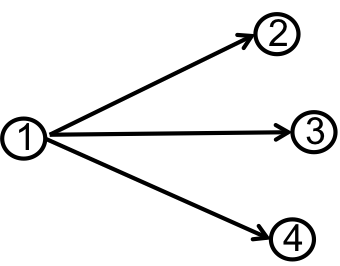
\includegraphics[width=0.2\textwidth]{facility_location}
\end{center}

\begin{enumerate}[(a)]
\item Find two different ways to enforce the requirement that if facility $1$ is closed, there is no flow out of facility $1$: one that uses 1 constraint, and one that uses 3 constraints.  

\medskip
\answerbox{c}{6cm}{3cm}  \hspace{.8cm} \answerbox{c}{6cm}{3cm}

\wordbox formulation \hspace{1.8cm}  \wordbox formulation

\medskip
According to our discussion,  one of these is the ``weak formulation'' and one is the ``strong formulation''.  Which is which?  Label accordingly.


\item  This bears out in practice.  The \wordbox formulation is has better performance in IP solvers on large problems.  (Although, professional-quality solvers will take care of this during pre-processing.)
\end{enumerate}
\end{problem}

\vfill
In summary:
\begin{tcolorbox}
Finding the convex hull of an integer program is the gold standard of IP formulations. That said, there are several issues with this:
	\begin{enumerate}
	\item Exponential number of constraints
	\item Potential numerical issues with tons of constraints
	\end{enumerate}
In general, we do not look for the convex hull. We do, however, use this idea to generate \textbf{cuts} when solving IPs.
\end{tcolorbox}


\section{Bounds for IPs}

In the next two class periods, we will look at ``branch-and-bound'', the algorithmic framework that most MIP (mixed-integer \emph{linear} programming) solvers use.  A critical component of this algorithm is producing bounds on the integer optimal solution.  

\subsection{Upper and lower bounds for IPs}
	
\begin{problem}
Suppose (P) is an IP with a maximizing objective function,
\[  \text{maximize } f(\mathbf{x}) = c_1 x_1 + c_2 x_2,  \]
where $c_1$ and $c_2$ are integers.  The feasible regions of (P) and (LP), the LP relaxation of (P), are pictured below.



\vspace{0.5cm}
\begin{center}
\begin{minipage}{6.5in}
\centering
\raisebox{-0.5\height}{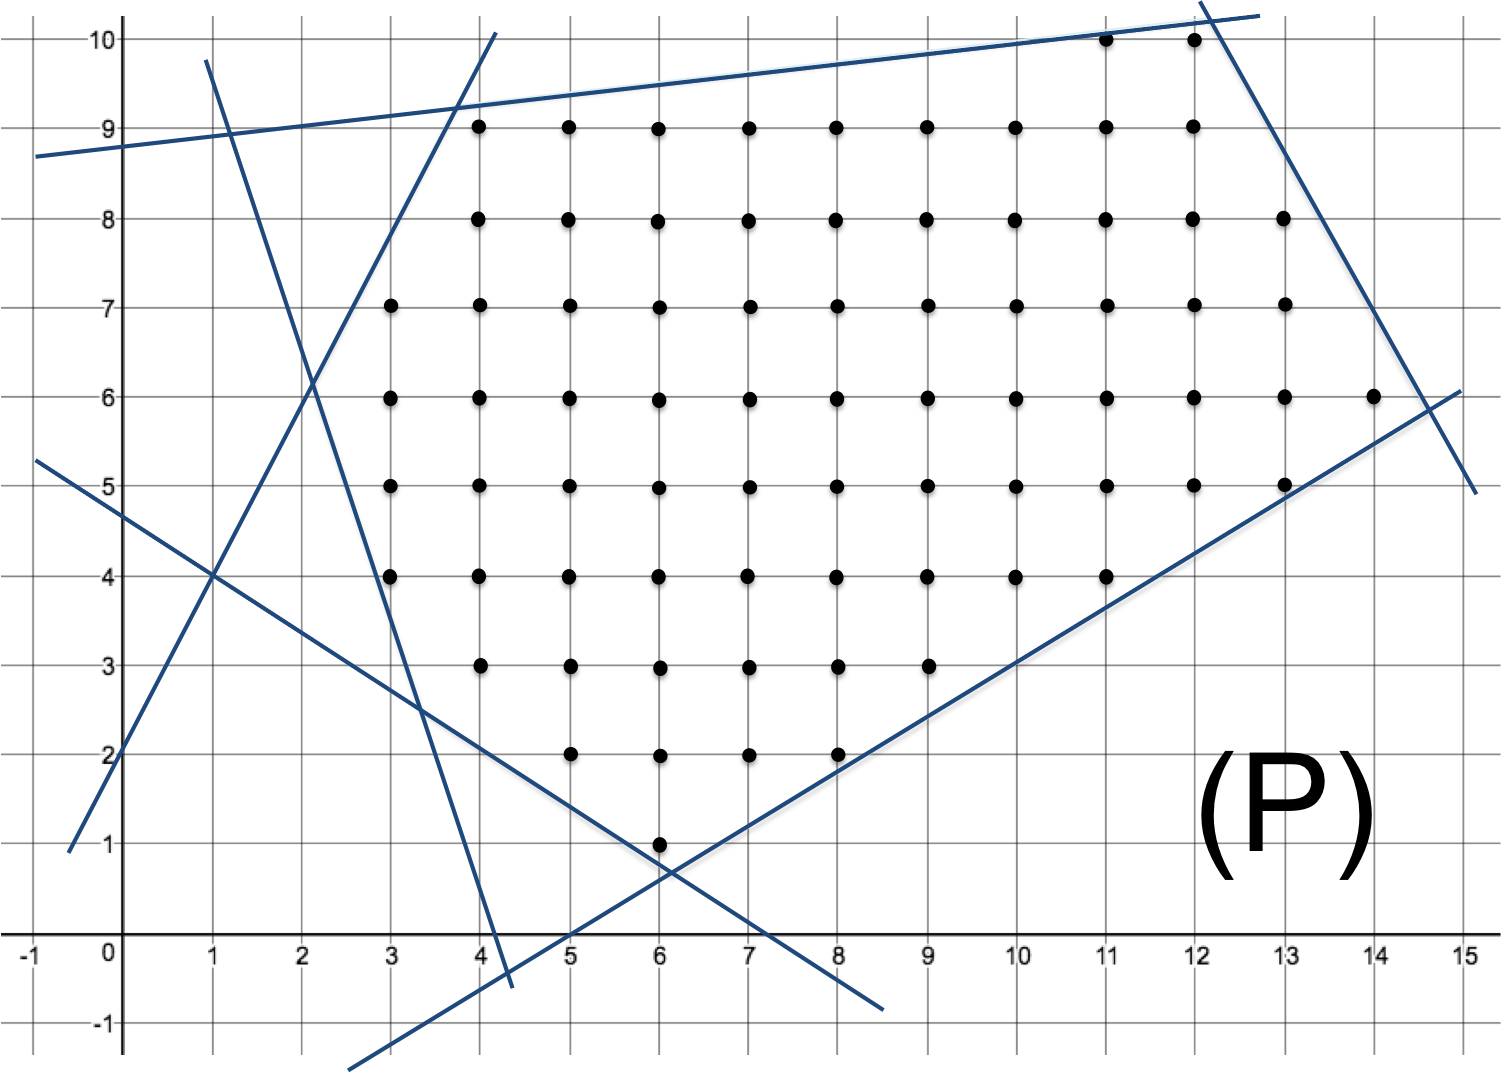
\includegraphics[width=0.4\textwidth]{P}}
\hspace*{0.2in}
\raisebox{-0.5\height}{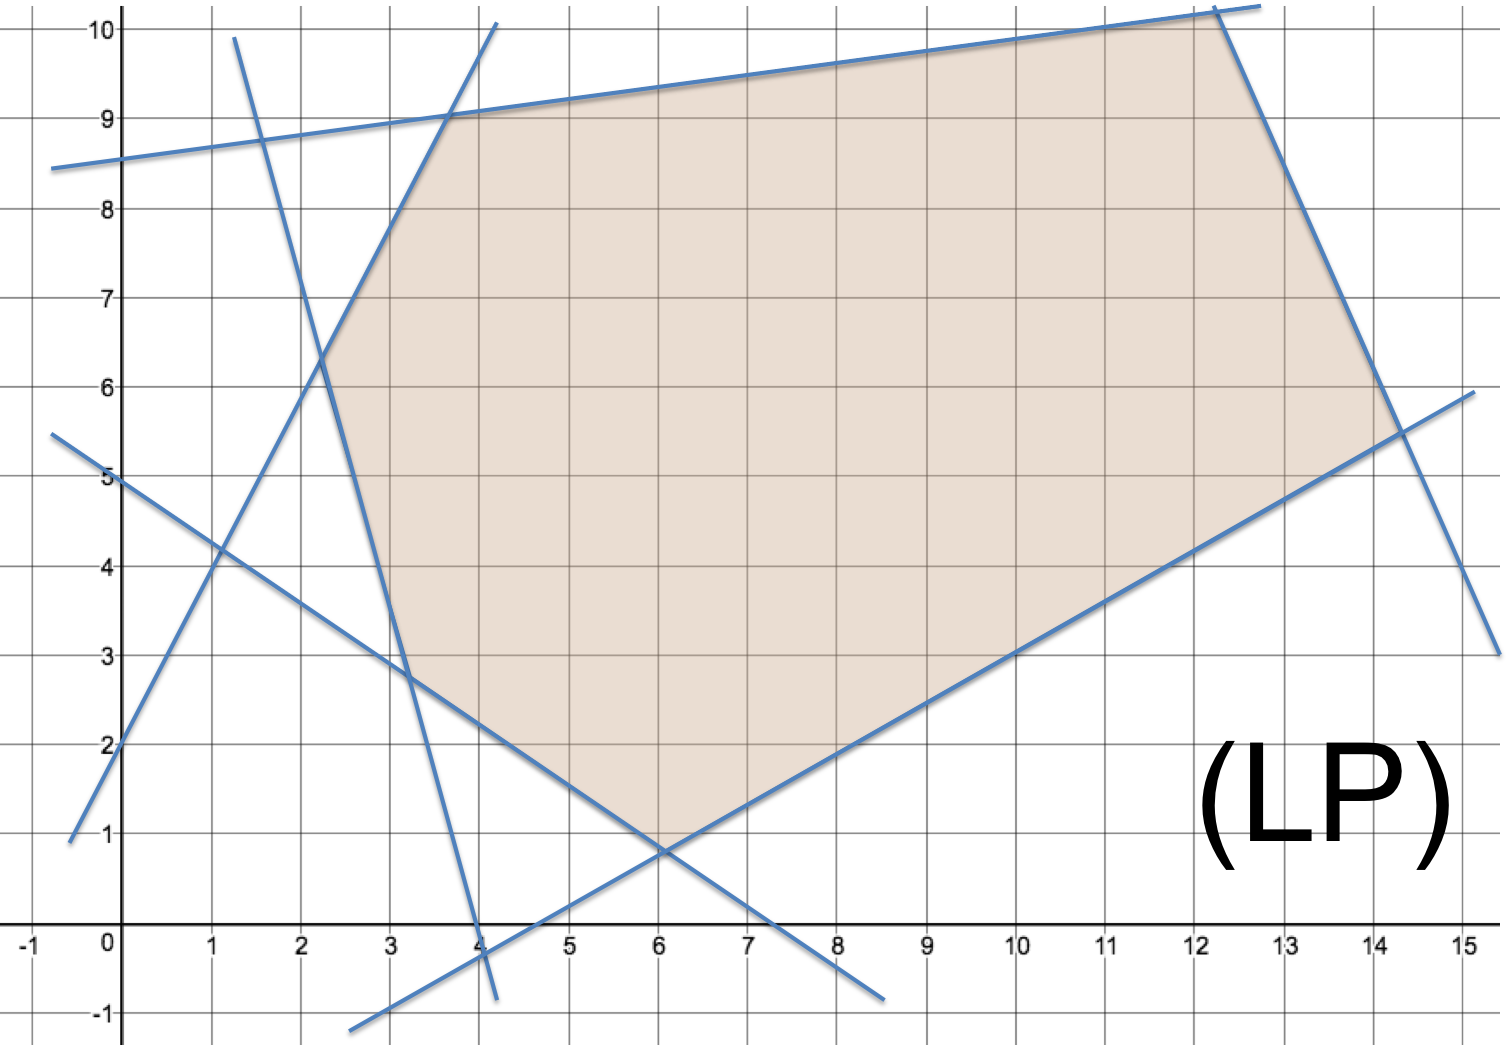
\includegraphics[width=0.4\textwidth]{LP}}
\end{minipage}
\end{center}


Let  $z^*$ be the optimal objective value of (P), which we want to find upper and lower bounds for as part of the branch and bound algorithm.

\begin{enumerate}[(a)]
\item    Suppose we solve the LP relaxation (LP) and get an optimal objective value of 83.9.  What can we say about $z^*$ relative to 83.9?  Explain.

\answerboxone{c}{1in}

\item We already stated that the $c_1$ and $c_2$ are integers.  What does that tell us about $z^*$?  Explain.  \emph{Hint:  Suppose $(x^*_1, x^*_2)$ is an optimal solution to (P).  What do we know about $x^*_1$ and  $x^*_2$?}

\answerboxone{c}{1in}

\item  Combining parts (a) and (b), find a better bound for $z^*$.  Explain.

\answerboxone{c}{1in}

\item  Now suppose that $\hat{\mathbf{x}} = (\hat{x}_1, \hat{x}_2)$, is some \emph{feasible} solution to (P) (not necessarily optimal).  What can we say about $f(\hat{x}) =  c_1 \hat{x}_1 + c_2 \hat{x}_2$ relative to $z^*$?  Explain.

\answerboxone{c}{1in}
\end{enumerate}
\end{problem}

\subsection{Better formulation leads to better (LP) bounds}

The quality of the bound obtained by solving the LP relaxation depends on the formulation:
\begin{center} 
A \textbf{tighter} formulation provides a \wordbox bound via its LP relaxation.
\end{center}

\subsection{Summary of IP bounds}

\begin{tcolorbox}
If (P) is a \textbf{maximizing} IP with integer objective coefficients and optimal objective value $z^*$,
\begin{itemize}
\item  If $z^*_{LP}$ is the optimal objective value to the LP relaxation of (P), then \catbox is a/an \wordbox bound on $z^*$.
\item  The objective value for \emph{any feasible} solution to (P) provides a/an \wordbox bound on $z^*$.
\end{itemize}
\end{tcolorbox}

\begin{tcolorbox}
If (P) is a \textbf{minimizing} IP with integer objective coefficients and optimal objective value $z^*$,
\begin{itemize}
\item  If $z^*_{LP}$ is the optimal objective value to the LP relaxation of (P), then \catbox is a/an \wordbox bound on $z^*$.
\item  The objective value for \emph{any feasible} solution to (P) provides a/an \wordbox bound on $z^*$.
\end{itemize}
\end{tcolorbox}








\end{document}

%\textbf{Fixed-Charge -- Linear Objective:}  Did you wonder why these were called the ``weak'' and ``strong'' formulations?  We compared these formulations on a very small problem.  Both formulations resulted in the same optimal solution, and both took about the same length of time.  What do you think will happen when we test these formulations on a larger problem? Why?  

%\answerboxfull{c}{2cm}

%Let's take a look at what happens when we solve a larger fixed-charge facility location problem with a \textbf{linear objective function} using \texttt{GLPK} (the \texttt{GUSEK} solver).  Record the results below.

%Weak formulation:

%\answerboxfull{c}{2cm}

%Strong formulation:

%\answerboxfull{c}{2cm}

%How can we explain this outcome?

%\answerboxfull{c}{2cm}

%The case of a linear objective function is well-studied in the context of many common problems.  This intelligence is \emph{built into most modern solvers}.

%\textbf{Fixed-Charge -- Nonlinear Objective:}   Current research focuses on \emph{nonlinear} problems.   In the presence of a \textbf{nonlinear objective function}:

%\begin{itemize}
%\item the optimal solution (IS or IS NOT) guaranteed to occur at a corner point;
%\item the \wordbox of the feasible region is more important than the boundary;
%\item we can omit constraints that don't ``cut-off'' much volume, to simplify a formulation.
%\end{itemize} 

%With a \wordbox objective function, the weak forcing constraints perform slightly better

%than the strong, due to a very similar volume and a smaller formulation.

